% 02/01 changed according to ref No.2
% 02/04 inserted Fig_s4
% 02/05 changed from .emf to n.png
% 02/06 changed according to ref No.2 (by Makimoto)

%%%%%%%%%%%%%%%
%   VWAP    %%
%%%%%%%%%%%%%%%

%\setcounter{section}{0}

\chapter{Optimal Slice of a VWAP Trade}\label{chap_s}


\begin{quote}
{\bf Abstract} \quad This chapter derives a static optimal execution strategy of a VWAP trade, in which the optimal execution strategy can be calculated by an iteration of a single variable optimization, rather than by a multivariable optimization.  Analytical solutions are derived in some cases.  We show that optimal execution times lag behind expected market trading volume distribution since price volatility tends to have a positive correlation with market trading volume.  In a basket trade, execution error can be reduced by spreading out execution times according to the correlation of price movement.  We confirm our theoretical results with actual trading data and simulations.
\vspace*{0.5cm}

\end{quote}


%%%%%%%%%%%%%%%%%
\section{Introduction}\label{sec_s1}
VWAP stands for volume-weighted average price during a certain trading period, and a VWAP trade refers a trade that uses VWAP as a benchmark.  This chapter analyzes optimal execution of a VWAP trade since little academic work can be found on this issue although VWAP has become an industry standard, and several studies have been made on optimal strategies for general trade execution.

VWAP trades are overtaking fixed-price trades in stock markets these days for several reasons.  First, foreign investors and individual investors reduce trading costs by VWAP trades.  For example, foreign investors are often forced to place large orders before the market opens due to the time lag.  In a fixed-price trade, brokers, who are generally risk averse, charge a large risk premium because of the size of the risk.  However, investors can save on the risk premium by using VWAP as a benchmark because market directional risk remains the investors' responsibility. 

Second, a block trade and determination of the option strike price require high price transparency, which can be achieved with a VWAP benchmark.  In a block and option trade, brokers try to cover their exposure to price movement risk as closely to a benchmark as possible in order to avoid possible losses.  If investors use a price at a fixed time in the future as a benchmark, the closing price for instance, brokers are forced to trade intensively towards closing, which results in a huge market impact, and burdens investors with considerable costs.  However, a VWAP benchmark can reduce the market impact of hedging trades and prevent manipulation of market prices.  

Third, VWAP orders can be used to evaluate traders' performance since the effect of market directional movement, which is considered to be noise in performance measurements, is excluded in comparisons with VWAP.  As a result, a number of institutional investors such as pension funds and mutual funds place VWAP orders. 

While investors can place fixed-price orders at any time they like, VWAP orders are gathered by brokers before a trading period starts.  Brokers then match buy and sell orders, and only the surplus is executed in the market.  Note that aggregated VWAP orders tend to involve various stocks and consist of a few large orders and numerous small orders due to the characteristics mentioned above.  Further, small orders for which buyers or sellers take the trouble to use a VWAP benchmark generally have low liquidity.

In executing market trades, a VWAP trader wishes to get the average execution price as close to the market VWAP as possible to avoid price movement risk.  To do so, a VWAP trader slices a whole trade into small executions and tries to spread the executions in a well-balanced manner over the trading period, which makes VWAP trades rather labor intensive.  Therefore, it often makes sense to build a standard strategy beforehand, and execute trades automatically according to it.  A standard strategy is especially good for small orders and orders with small weights in a basket trade whose economic impact is small.  Consequently, this chapter focuses on the optimal strategy for automatic execution of small VWAP orders with low liquidity.  

As the investment business becomes increasingly competitive and understanding of the market microstructure improves, trading costs attract greater attention from both practitioners and academic researchers.  As a consequence, several studies have examined optimal trade execution strategy.  For example, Harris and Hasbrouck (1996) and Parlour (1998) analyze the choice of market and limit orders, and Bertsimas and Lo (1998) and Chapter \ref{chap_b} of this study derive an optimal slicing strategy for block trades.  Although this chapter has similar objectives to those of preceding studies, both market price and trading volume are stochastic in a VWAP trade, while only the price process is stochastic in a block trade.

Numerous studies have been done on the relationship between price volatility and market trading volume since Clark's (1973) seminal paper, including Epps and Epps (1976), Tauchen and Pitts (1983).  Karpoff (1987) summarizes these results, and Andersen (1996) proposes a modified model.  These studies, in general, support the existence of a positive correlation between price volatility and market trading volume and the autocorrelation of themselves because surprising news boosts both price volatility and market trading volume.  Besides, Jain and Joh (1988), Admati and Pfleiderer (1988), Foster and Viswanathan (1990), and Chan et al.~(1995) study intraday data and find a ``U-shaped effect," i.e., within a single day, price volatility and market trading volume tend to be higher at the opening and closing than in the middle of a trading session.  Naturally, our VWAP model reflects these findings.

Dynamic optimization, in which the actual trading strategy might be changed as new information arrives, is certainly a potential VWAP execution strategy.  However, static optimization without strategy changes works well enough, especially for small VWAP orders with low liquidity.  This is because observed variables such as the price volatility and market trading volume of stocks with low liquidity may contain statistical errors too large to be used in forecasting, and therefore, dynamic optimization is considered to be inaccurate.  For example, when market trading volume suddenly surges, it is difficult to predict whether high market trading volume is temporary or permanent even judging qualitatively.  In spite of inaccuracy and trouble related to dynamic optimization, the impact of small orders on cost efficiency is insignificant.  Consequently, static optimization is considered a reasonable alternative. 

Further, a static optimal execution strategy can be used as a benchmark for a dynamic execution strategy.  A strategy change can be evaluated by comparing the realized cost to that of a static optimal execution strategy.

For these reasons, this chapter focuses on the static optimal execution strategy of a VWAP trade.  Specifically, optimal trade decisions are made before the trading period, based on traders' expectations regarding price volatility, market trading volume, and the correlation between these values at different time of the day.  No revision is allowed in the middle of the day after the true market trading volume is observed.  

The rest of this chapter is organized as follows.  Section \ref{sec_s2} formulizes the optimal strategy.  Section \ref{sec_s3} derives solutions for single-stock cases, analyzes characteristics of the optimal strategy, and tests them against historical data.  Section \ref{sec_s4} analyzes a multiple-stock case.  Finally, Section \ref{sec_s5} concludes the analysis.

%%%%%%%%%%%%%%%%%%%%%%%
\section{Formulization of the Optimal Slicing}\label{sec_s2}
Imagine a case in which a trader buys a certain number of shares and
tries to get the average purchase price as close as possible to the
market VWAP during the trading period from time 0 to time $T$.    Let
$(\Omega, \calF, Q)$ be a probability space with a filtration
$\{ \calF_t \}$, which satisfies usual conditions.  Let $V(t)$
denote the accumulated market trading volume at time $t$ excluding the
trader's, and $v(t)$ the trader's accumulated trading volume.
 Here, $\{ V(t) \}$ is an $\{ \calF_t \}$-adapted process in $L^2$ space, and $v(t)$ is a controllable variable.  At time 0, the trader knows $v(0)=V(0)=0$ and the whole trade size $v(T)$ which is given exogenously, but not $V(t)$ for $t>0$.  We do not allow sell orders, and therefore, $v(t)$ is a non-negative increasing function as well as $V(t)$.  Further, minimum trading unit is given exogenously and normalized to one for simplicity, which makes $V(t)$ and $v(t)$ step functions, and we assume left continuous. 

Let $\{ P(s) \}$ denote a non-negative $\{ \calF_t \}$-adapted stock price process in $L^2$ space.  A trader's own VWAP is expressed as
\[
  vwap=\frac{\int_0^T P(s) dv(s)}{v(T)}.
\]

Also, the market VWAP is 
\[
  VWAP=\frac{\int_0^T P(s)d\{V(s)+v(s)\}}{V(T)+v(T)}=\frac{\int_0^T P(s)dV(s)+v(T) \times vwap}{V(T)+v(T)}.
\]
As we have mentioned, a VWAP trader tries to get his VWAP as close to the market VWAP as possible.  Generally speaking, the market impact of a VWAP trade is insignificant because the whole trade is divided into small executions.  Therefore, this chapter ignores the market impact effect and minimizes the expected squared error of the VWAP execution due to price movement.  Mathematically, our objective is represented as
\[
  \min_{v(t)} \ex{(VWAP-vwap)^2}.
\]
The following proposition holds regarding the expected squared error of the VWAP execution.

\begin{proposition}\label{prop_s1}
 \quad The expected squared error of the VWAP execution is calculated as 
\[
  W \ex{\left\{\int_0^T (X(t)-x(t))dP(t)\right\}^2}+\cov{\left(\frac{V(T)}{V(T)+v(T)}\right)^2}{\left\{\int_0^T (X(t)-x(t))dP(t)\right\}^2}
\]
where 
\[
 X(t)=\frac{V(T)-V(t)}{V(T)}, \quad x(t)=\frac{v(T)-v(t)}{v(T)},
 \quad W=\ex{\left(\frac{V(T)}{V(T)+v(T)}\right)^2}.
\]
\end{proposition}

\begin{proof}
  See Section \ref{sec_sappendix}.
\end{proof}

In this proposition, $X(t)$ and $x(t)$ stand for the ratio of remaining trading volume of the market and of the trader, respectively, and both of them are left continuous decreasing step functions.  We call $x(t)$ an execution strategy function henceforth.

Further, when $V(T)$ is sufficiently large compared to $v(T)$, $\frac{V(T)}{V(T)+v(T)}$ has a value close to one, which makes its variation small and the covariance term negligible.  Thus, we make the following assumption.

\begin{assumption}\label{ass_s1}
\quad The expected squared error can be approximated as
\begin{equation}\label{eq_s1}
  W \ex{\left\{\int_0^T (X(t)-x(t))dP(t)\right\}^2}.
\end{equation}
\end{assumption}

Since this formula is still too complicated to generate implications, further assumptions are made which are considered reasonable based on standard theories and empirical analyses.  First, the stock price process is assumed to follow a Brownian motion, similar to standard option pricing theory.  The drift term is considered to be zero because the time frame is short.  Second, according to the ``Mixture of Distribution Hypothesis" by Clark (1973) and empirical analysis by Jain and Joh (1988), there exists a relationship between price volatility and market trading volume which can be written as follows.

\begin{assumption}\label{ass_s2}
 \quad The stock price process is represented as
\[
  dP(t)=\sigma(t,V(t))dB(t),
\]
in which $\sigma(t,V(t))$ is a positive $\{ \calF_t \}$-adapted process in $L^2$ space, and $B(t)$ is a standard Brownian motion on $(\Omega, \calF, Q)$.  
\end{assumption}

 We can assume that the probability of a negative $P(t)$ is negligible because the time frame is short.

Under these assumptions, (\ref{eq_s1}) becomes
\begin{equation}\label{eq_s2}
  W \int_0^T \ex{\sigma(t,V)^2(X(t)-x(t))^2} dt.
\end{equation}
This equation gives great insight into the difficulty of certain VWAP trades: a trade with a small expected squared error is a trade large enough to make $W$ small and $w(t)$ smooth, with a stable market trading volume distribution over time, and with low price volatility.

Since our objective is to minimize the value of (\ref{eq_s2}), our problem can be further modified as,
\begin{eqnarray}
    \lefteqn{\mbox{min} \int_0^T \ex{\sigma(t,V)^2(X(t)-x(t))^2} dt} \nonumber \\
    & = & \int_0^T \ex{\sigma(t,V)^2X(t)^2}dt+ \min\int_0^T \{-2\ex{\sigma(t,V)^2X(t)}x(t)+ \ex{\sigma(t,V)^2}x(t)^2]\}dt \nonumber \\
    & = & \int_0^T \left\{ \ex{\sigma(t,V)^2X(t)^2}-\frac{\ex{\sigma(t,V)^2X(t)}^2}{\ex{\sigma(t,V)^2}} \right\} dt \nonumber \\
    &   & + \min \int_0^T \left\{ \frac{\ex{\sigma(t,V)^2X(t)}}{\ex{\sigma(t,V)^2}}-x(t)\right\}^2\ex{\sigma(t,V)^2} dt \label{eq_s3}
\end{eqnarray}
in which $x(t)$ is a controllable variable and others are given parameters.

In practice, expectations of $\sigma(t,V)^2$ and $X(t)$ vary gradually across time except at scheduled events such as batch auctions and news announcements.  Therefore, $\displaystyle \frac{\ex{\sigma(t,V)^2X(t)}}{\ex{\sigma(t,V)^2}}$ in (\ref{eq_s3}) can be assumed to be continuous almost everywhere with finite jumps.  Also, we can assume that $\displaystyle \frac{\ex{\sigma(t,V)^2X(t)}}{\ex{\sigma(t,V)^2}}$ is left continuous without loss of generality, in the same way as $X(t)$ and $x(t)$.

Let $t_k \quad (k=1,\cdots,v(T))$ denote $v(T)$ of execution times, and define $t_0=0$ and $t_{v(T)+1}=T$.  Then, $x(t)$ is a step function with $v(T)+1$ values as follows.
\begin{equation}\label{eq_s4}
  x(t)=1-\frac{k}{v(T)} \quad \mbox{if} \quad t_k < t \leq t_{k+1} \quad (k=0,\cdots,v(T)).
\end{equation}
Therefore, determination of the optimal execution strategy function $x^*(t)$ is equivalent to determination of optimal execution times $\{t_k^*\}$.  Further, a careful examination of (\ref{eq_s3}) reveals that this problem is considered to be an issue of how to approximate a function, continuous almost everywhere, with a step function as in Figure \ref{fg_s1}.

\begin{figure}[htbp]
\begin{center}
 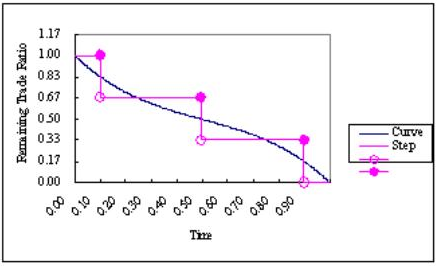
\includegraphics[width=10cm,height=5cm]{fg_s1n.png}
\end{center}
\caption[Image of $\displaystyle \frac{\ex{\sigma(t,V)^2X(t)}}{\ex{\sigma(t,V)^2}}$ and $x(t)$]
{{\bf Image of $\displaystyle \frac{\ex{\sigma(t,V)^2X(t)}}{\ex{\sigma(t,V)^2}}$ and $x(t)$} (Curve:
$\displaystyle \frac{\ex{\sigma(t,V)^2X(t)}}{\ex{\sigma(t,V)^2}}$, Step: $x(t)$).
 \quad Our problem is considered to be an issue of how to approximate
$\displaystyle \frac{\ex{\sigma(t,V)^2X(t)}}{\ex{\sigma(t,V)^2}}$, a function differentiable almost everywhere with
finite jumps, with $x(t)$, a left continuous step function with $v(T)+1$ values.}\label{fg_s1}
\end{figure}

It is possible that $t_k^*$ is equal to $t_{k+1}^*$ where $\displaystyle \frac{\ex{\sigma(t,V)^2X(t)}}{\ex{\sigma(t,V)^2}}$ jumps at batch auctions.  In this case, multiple units are executed simultaneously.  This does not detract from our argument since we ignore trading costs, including the market impact.  Note that if $v(T)$ is large enough, $x^*(t)$ can be approximated by
\[
\displaystyle x^*(t) \approx \frac{\ex{\sigma(t,V)^2X(t)}}{\ex{\sigma(t,V)^2}}.
\]

Mathematically, the following proposition holds.

\begin{proposition}\label{prop_s2}
\begin{eqnarray}
    &   & \min\int_0^T \{-2\ex{\sigma(t,V)^2X(t)}x(t)+ \ex{\sigma(t,V)^2}x(t)^2]\}dt\nonumber \\
    & = & \min \sum_{k=1}^{v(T)} \int_0^{t_k} \left[ \left\{ -\frac{2\ex{\sigma(t,V)^2X(t)}}{v(T)\ex{\sigma(t,V)^2}}+\frac{2(v(T)-k)+1}{v(T)^2}\right\}\ex{\sigma(t,V)^2}\right]dt. \label{eq_s5}
\end{eqnarray}
\end{proposition}

\begin{proof}
  See Section \ref{sec_sappendix}.
\end{proof}

Note that we can optimize each $t_k$ separately since it appears only as the upper bound of the integral on the right hand side of (\ref{eq_s5}).  The specific solution is derived in the following section.

%%%%%%%%%%%%%%%%
\section{Derivation of the Optimal Strategy: Single-Stock Case}\label{sec_s3}
In this section, we derive solutions both when price volatility is uncorrelated and correlated with market trading volume, and compare these results.

\subsection{Uncorrelated Case: $\sigma$ is uncorrelated with $V$}
In this case, the optimal execution strategy can be solved explicitly as the following proposition.

\begin{proposition}\label{prop_s3}
 \quad Under Assumptions \ref{ass_s1} and \ref{ass_s2}, and if price volatility is uncorrelated with market trading volume, optimal execution times $\{t_k^*\}$ are determined to satisfy 
\[
  \ex{X(t_k^*)} \geq \frac{2(v(T)-k)+1}{2v(T)} \geq \lim_{t \downarrow t_k^*} \ex{X(t)}.
\]
Further, the optimal execution strategy function $x^*(t)$ is solved as
\[
  x^*(t)=\frac{\lfloor (2v(T)\ex{X(t)}+1)/2 \rfloor}{v(T)},
\]
where $\lfloor x \rfloor$ represents the integer part of $x$.
\end{proposition}

\begin{proof}
  See Section \ref{sec_sappendix}.
\end{proof}

Therefore, $\{t_k^*\}$ is determined only by $\ex{X(t)}$, and is independent of expectations regarding the magnitude and term structure of price volatility.  Note that $x^*(t)$ is solved directly without solving $\{t_k^*\}$.

In practice, it used to be common to divide trading periods into equal time intervals and to allocate executions proportional to $\ex{X(t)}$.  However, this strategy (Old Strategy henceforth) comes with attendant problems, namely that as intervals are shortened in an attempt to track market trading volume more closely, more orders are placed at the opening and closing when instantaneous market trading volume is larger than in the middle of the trading session.  In contrast, our optimal strategy (New Strategy henceforth) is derived by dividing $\ex{X(t)}$ into the number of shares and executing at the middle of $\ex{X(t)}$ in each interval.  In other words, the New Strategy takes price movement risk into account and minimizes time differences in order execution.  Note that the interval with high market trading volume is not necessarily the optimal execution time.  Consequently, the New Strategy provides not only an optimal slice with the least expected squared error but also an unbiased slice for any orders even if the time intervals are infinitesimally small.

Next, we confirm our theoretical results empirically, using actual intraday data from the Tokyo Stock Exchange provided by Nikkei Quick Information Co. Ltd.  All empirical analyses in this chapter are based on trading data from October 2000 to March 2001 on the 10 stocks with the largest market capitalization.  Data from December 29, 2000 and January 4, 2001 are excluded since there was no afternoon session on these days.  We chose these large stocks in order to retain statistical accuracy since their ticks are frequent and stable.  We believe that results can be applied to other stocks since the relationship between price volatility and market trading volume is ubiquitous for all stocks as Chan et al. (1995) point out.  

Figure \ref{fg_s2} shows the standard deviation of VWAP execution errors using the Old Strategy and the New Strategy when the whole day is divided into nine intervals of 30 minutes each.  Specifically, we first estimate $\ex{X(t)}$ of each stock as the average of past trading data.  Then, in the Old Strategy, fixed number of executions are allocated proportional to the increment of $\ex{X(t)}$ for the nine intervals with the smallest rounding errors.  In the New Strategy, executions are allocated by the prescribed method.  For comparison, we assume that trades are executed at VWAP of each interval in both Old and New Strategy.  This allocation is fixed during the whole sample period, and VWAP execution errors are calculated everyday.  Finally, standard deviation of VWAP execution errors is calculated over sample stocks and dates.

According to Figure \ref{fg_s2}, the superiority of the New Strategy, especially for small orders, is evident.  The superiority is more conspicuous when time intervals are shortened, although we do not show the result here.

\begin{figure}[htbp]
\begin{center}
 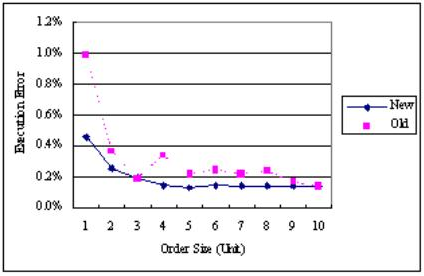
\includegraphics[width=10cm,height=6cm]{fg_s2n.png}
\end{center}
\caption[Comparison of execution strategies]
{{\bf Comparison of execution strategies.}
 \quad This graph shows the standard deviation of VWAP execution errors using the {\it old strategy} and the {\it new strategy}
($y$-axis) for different order sizes ($x$-axis) when the whole day is divided into nine intervals of 30 minutes
each.
 The superiority of the new strategy, especially for small orders, is evident.}\label{fg_s2}
\end{figure}


\subsection{ Correlated Case: $\sigma$ is a function of $V$}
In this case, the integrand in (\ref{eq_s5}) is not necessarily increasing. However, what we have to do is essentially the same; to find the upper bounds of the integrals one by one so as to minimize the area between the straight line and the curved line in Figure \ref{fg_s3}: negative if the curved line is below the straight line, positive if the curved line is above the straight line.  As we can see in Figure \ref{fg_s3}, the upper bounds fall on one of the countable points where the curved line rises to intersect the straight line (A or G for $t_k^*$, and B or H for $t_{k+1}^*$ in Figure \ref{fg_s3}).  Therefore, we have only to evaluate the integral at these points and choose one that minimizes the integral.

\begin{figure}[htbp]
\begin{center}
 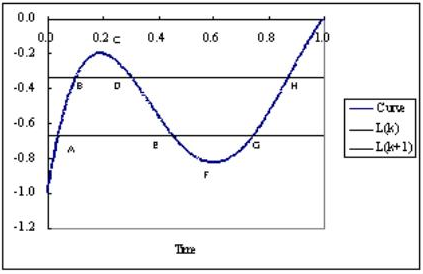
\includegraphics[width=10cm,height=6cm]{fg_s3n.png}
\end{center}
\caption[Optimization image]
{{\bf Optimization image} (curve: $\displaystyle \frac{\ex{\sigma(t,V)^2X(t)}}{\ex{\sigma(t,V)^2}}$, $L(k)$:
$\displaystyle -\frac{v(T)-k+1/2}{v(T)}$, $L(k+1)$: $\displaystyle -\frac{v(T)-(k+1)+1/2}{v(T)}$).
 \quad Although the integrand is not necessarily increasing, we still want to find the upper bounds of integrals one
 by one so as to minimize the area between the straight line and the curved line.
 It turns out that such a point falls on one of the countable points where the curved line rises to intersect
the straight line (A or G for $t_k^*$, and B or H for $t_{k+1}^*$).
 Therefore, we have only to evaluate the integral at these points and choose one that minimizes the
integral.}\label{fg_s3}
\end{figure}


Note that $t_k^*$ and $t_{k+1}^*$ chosen separately in the above procedure always satisfy $t_k^* \leq t_{k+1}^*$.  This is obvious when $t_k^*$ falls on A.  If $t_k^*$ falls on G, $\mbox{Area(ACE)} < \mbox{Area(EFG)}$ holds.  Together with $\mbox{Area(BCD)} < \mbox{Area(ACE)}$ and $\mbox{Area(EFG)} < \mbox{Area(DFH)}$, $\mbox{Area(BCD)} < \mbox{Area(DFH)}$.  Consequently, $t_{k+1}^*$ falls on H and is larger than $t_k^*$.

As a matter of fact, $\displaystyle \frac{\ex{\sigma(t,V)^2X(t)}}{\ex{\sigma(t,V)^2}}$ is usually stable and monotone decreasing in practice, as we confirm with actual data later.  Therefore, we make the following assumption in the rest of Section \ref{sec_s3}.

\begin{assumption}\label{ass_s3}
 \quad $\displaystyle \frac{\ex{\sigma(t,V)^2X(t)}}{\ex{\sigma(t,V)^2}}$ is monotone decreasing.
\end{assumption}

Under this assumption, the term in the bracket in (\ref{eq_s5})
\[
  \left\{-\frac{2\ex{\sigma(t,V)^2X(t)}}{v(T)\ex{\sigma(t,V)^2}}+\frac{2(v(T)-k)+1}{v(T)^2}\right\}
\]
is increasing and turns from negative to positive just once.  Further, even if the integrand itself  
\[
  \left\{-\frac{2\ex{\sigma(t,V)^2X(t)}}{v(T)\ex{\sigma(t,V)^2}}+\frac{2(v(T)-k)+1}{v(T)^2}\right\}\ex{\sigma(t,V)^2}
\]
is not increasing, the integrand turns from negative to positive only once since $E[\sigma(t,V)^2]$ is positive.  Consequently, we can obtain the optimal solution explicitly at such a unique point just as in the Uncorrelated Case, and the following proposition holds.  

\begin{proposition}\label{prop_s4}
 \quad Under Assumptions \ref{ass_s1} -- \ref{ass_s3}, and if price volatility is correlated with market trading volume, optimal execution times $\{t_k^*\}$ are determined to satisfy 
\[
  \ex{\sigma(t_k^*,V)^2X(t_k^*)} \geq \frac{2(v(T)-k)+1}{2v(T)}\ex{\sigma(t_k^*,V)^2} \geq \lim_{t \downarrow t_k^*} \ex{\sigma(t,V)^2X(t)}.
\]
Further, the optimal execution strategy function $x^*(t)$ is solved as
\[
  x(t)=\frac{\lfloor (\frac{2v(T)\ex{\sigma(t,V)^2 X(t)}}{\ex{\sigma(t,V)^2}}+1)/2 \rfloor}{v(T)}
\]
where $\lfloor x \rfloor$ represents the integer part of $x$.

\end{proposition}

According to Clark (1973), Jain and Joh (1988), and others, $\sigma(t,V)$ is considered to be an increasing function of market trading volume, or equivalently, an increment of $V(t)$ because surprising news boosts both $\sigma(t,V)$ and the increment of $V(t)$.  Also, since the increment of $V(t)$ tends to have a positive autocorrelation, $X(t)$ is an increasing function of the increment of $V(t)$.  Therefore, in general, the correlation between $\sigma(t,V)^2$ and $X(t)$ is positive, or equivalently, $\ex{\sigma(t,V)^2X(t)}>\ex{\sigma(t,V)^2}\ex{X(t)}$.  Consequently, $x^*(t)$ in the Correlated Case tends to become larger than in the Uncorrelated Case, which delays trade execution.  This is because once price volatility and market trading volume surge, traders have to make considerable trades to track market trading volume while execution times do not matter when these parameters remain small throughout the day.

There might be two approaches to check the monotonicity of $\displaystyle \frac{\ex{\sigma(t,V)^2X(t)}}{\ex{\sigma(t,V)^2}}$: theoretical and empirical.  In the theoretical approach, we can find sufficient conditions with existing models such as Clark (1973), Admati and Pfleiderer (1988), Andersen (1996), and others, and check that actual data satisfies such conditions.  While these conditions may take various forms, depending on parameter specifications in the models, their implications are similar: stable correlation, reasonable volatility, etc.  On the other hand, we can show the same results in the empirical approach without assuming any specific models.  Since the empirical approach is more robust, we check with past data that actual $\displaystyle \frac{\ex{\sigma(t,V)^2X(t)}}{\ex{\sigma(t,V)^2}}$ is indeed decreasing.

Table \ref{table_s1} shows the optimal allocation ratio of the VWAP execution for individual stocks in the Correlated Case, using the previous 10-stock trading data.  Prices are normalized so that those at the end of March are one.  Also, $v(t)$ is assumed to be large enough that $\displaystyle x^*(t) \approx \frac{\ex{\sigma(t,V)^2X(t)}}{\ex{\sigma(t,V)^2}}$.  $x^*(t)$ here is calculated from the average of $\sigma(t,V)^2X(t)$, and $\sigma(t,V)^2$ over the sample period.  Specifically, let $P_{d,t}$ and $V_{d,t}$ denote price and accumulated market trading volume in $d^{th}$ day $t^{th}$ interval ($d=1,\cdots,D$, $t=1,\cdots,T$).  Price change can be represented as 
\[
  \Delta P_{d,t} = \left\{
  \begin{array}{ll}
   P_{d,t}-P_{d,j-1}, \quad \mbox{for} \quad t=2,\cdots,T, \\
   P_{d,1}-P_{d-1,T}, \quad \mbox{for} \quad t=1
  \end{array}
  \right.
\]
and realized ratio of remaining trading volume as $\displaystyle X_{d,t}=\frac{V_{d,T}-V_{d,t-1}}{V_{d,T}}$.  We estimate $\ex{\sigma(t,V)^2X(t)}$ as $\displaystyle \frac{1}{D} \sum_{d=1}^D \Delta P_{d,t}^2X_{d,t}$, and estimate $\ex{\sigma(t,V)^2}$ as $\displaystyle \frac{1}{D} \sum_{d=1}^D \Delta P_{d,t}^2$.  Let $x_t^*$ denote the optimal ratio of remaining execution in the $t^{th}$ interval, then the optimal allocation ratio of the VWAP execution is given as $-(x_{t+1}^*-x_t^*)$.

\begin{table}[htbp]
\begin{center}
\begin{tabular}{|l|ccccccccc|} \hline
 Period & 1 & 2 & 3 & 4 & 5 & 6 & 7 & 8 & 9 \\ \hline
 Takeda & 0.22 & 0.09 & 0.07 & 0.10 & 0.14 & 0.04 & 0.09 & 0.07 & 0.17 \\
 Matsushita & 0.22 & 0.09 & 0.07 & 0.10 & 0.14 & 0.04 & 0.09 & 0.07 & 0.17 \\
 Sony & 0.21 & 0.09 & 0.10 & 0.09 & 0.11 & 0.07 & 0.06 & 0.10 & 0.16 \\
 Toyota & 0.23 & 0.04 & 0.12 & 0.05 & 0.13 & 0.09 & 0.06 & 0.01 & 0.27 \\
 Honda & 0.21 & 0.10 & 0.09 & 0.09 & 0.12 & 0.03 & 0.09 & 0.09 & 0.18 \\
 Mizuho & 0.19 & 0.08 & 0.08 & 0.09 & 0.11 & 0.10 & 0.08 & 0.08 & 0.18 \\
 Tokyo-Mitsubishi & 0.21 & 0.06 & 0.09 & 0.06 & 0.13 & 0.02 & 0.14 & 0.08 & 0.20 \\
 Nomura & 0.22 & 0.09 & 0.08 & 0.08 & 0.13 & 0.07 & 0.09 & 0.09 & 0.15 \\
 NTT & 0.21 & 0.08 & 0.09 & 0.07 & 0.12 & 0.06 & 0.10 & 0.07 & 0.21 \\
 NTT Docomo & 0.19 & 0.11 & 0.11 & 0.08 & 0.10 & 0.09 & 0.05 & 0.09 & 0.18 \\ \hline
\end{tabular}
\end{center}
\caption[Optimal allocation ratio of execution]{{\bf Optimal allocation ratio of execution.} \quad This table shows the optimal allocation ratio of the VWAP execution for individual stocks in the correlated case, using the previous 10 stock trading data.
  $v(t)$ is assumed to be large enough that ${\displaystyle x^*(t) \approx
\frac{\ex{\sigma(t,V)^2 X(t)}}{\ex{\sigma(t,V)^2}}}$.
 $X^*(t)$ here is calculated from the average of $\sigma(t,V)^2 X(t)$ and $\sigma(t,V)^2$ over the sampling period.
 As we expected, all the optimal allocation ratios of execution in the correlated case are positive, which means
${\displaystyle \frac{\ex{\sigma(t,V)^2 X(t)}}{\ex{\sigma(t,V)^2}}}$ is indeed monotone decreasing.}\label{table_s1}
\end{table}

As expected, all of the optimal execution allocation ratios of execution in Table \ref{table_s1} are positive, which means $\displaystyle \frac{\ex{\sigma(t,V)^2X(t)}}{\ex{\sigma(t,V)^2}}$ is indeed monotone decreasing.

Also, Figure \ref{fg_s4} shows the average of $x^*(t)$, which coincides with $\ex{X(t)}$ in the Uncorrelated Case and $\displaystyle \frac{\ex{\sigma(t,V)^2X(t)}}{\ex{\sigma(t,V)^2}}$ in the Correlated Case.  $\ex{X(t)}$ here is also estimated as an average over the sample period.  

We can see that $x^*(t)$ in the Correlated Case is, in fact, larger than in the Uncorrelated Case, which delays trade execution.  Besides, according to the same data, standard deviations of VWAP execution error are 0.127\% in the Uncorrelated Case and 0.119\% in the Correlated Case, which shows that a VWAP trade can be executed more accurately by taking into account the correlation between price volatility and market trading volume.

Main sources of these errors are considered to be statistical errors in estimating parameters and stochastic changes of parameters.  Regarding the statistical errors, empirical studies such as Uno and Yamada (1993) and Jain and Joh (1988) report that the parameters of the market impact coefficents, the price volatility, and the market trading volume are rather stable.  Regarding stochastic changes, execution errors can be reduced by dynamic optimization in Chapter \ref{chap_d}.  In practice, we further suffer price changes within the interval and discritization errors due to the minimum trading unit, both of which are considered to be proportional to the price volatility.

\begin{figure}[htbp]
\begin{center}
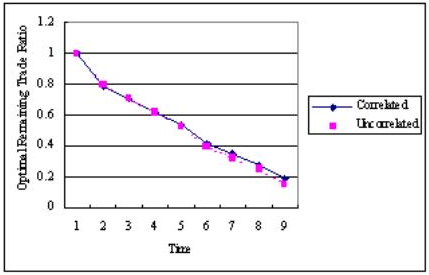
\includegraphics[width=10cm,height=6cm]{fg_s4n.png}
\end{center}
\caption[Comparison of average optimal execution strategy functions]
{{\bf Comparison of average optimal execution strategy functions.}
 \quad This graph shows the average of $x^*(t)$, which coincides with $\ex{X(t)}$ in the uncorrelated case and
$\displaystyle \frac{\ex{\sigma(t,V)^2X(t)}}{\ex{\sigma(t,V)^2}}$ in the correlated case.
 We can see that $x^*(t)$ in the correlated case is, in fact, larger than in the uncorrelated case, which delays trade
execution.}\label{fg_s4}
\end{figure}

%%%%%%%%%%%%%%%%%%%%%%%
\section{Derivation of the Optimal Strategy: Multiple-Stock Case}\label{sec_s4}
\subsection{Formulization of the Optimal Slicing}
Imagine a case with $N$ stocks.  Price, price volatility, the accumulated trading volume of the market and the trader, etc.\ of $i^{th}$ stock are represented by subscripts: $P_i(t)$, $\sigma_i(t)$, $V_i(t)$, $v_i(t)$, respectively, and satisfy similar conditions as in single-stock case.  Also, let $t_{ik} \quad (i=1,\cdots,N, k=1,\cdots,v_i(T))$ denote $v_i(T)$ of execution times of $i^{th}$ stock.   Further, define the weights of $i^{th}$ stock in the whole trade as
\[
   w_i=\frac{v_i(T)}{\sum_{j=1}^N v_j(T)}.
\]
The VWAP of the whole trade can be defined as the weighted average of the individual VWAP.  In this case, the following equation holds as Proposition \ref{prop_s1} in the single-stock case,
\begin{eqnarray*}
  \lefteqn{\ex{\{\sum_{i=1}^N w_i(VWAP_i-vwap_i)\}^2}} \\
  & = & \sum_{i=1}^N \sum_{j=1}^N W_{ij} \ex{\int_0^T (X_i(t)-x_i(t))dP_i(t)\int_0^T (X_j(t)-x_j(t))dP_j(t)} \\
  &   & + \cov{w_i\left(\frac{V_i(T)}{V_i(T)+v_i(T)}\right)w_j\left(\frac{V_j(T)}{V_j(T)+v_j(T)}\right)}{\int_0^T (X_i(t)-x_i(t)dP_i(t)\int_0^T (X_j(t)-x_j(t))dP_j(t)}
\end{eqnarray*}
where
\[
  X_i(t)=\frac{V_i(T)-V_i(t)}{V_i(T)}, \quad x_i(t)=\frac{v_i(T)-v_i(t)}{v_i(T)}, \quad W_{ij}=\ex{w_i\left(\frac{V_i(T)}{V_i(T)+v_i(T)}\right)w_j\left(\frac{V_j(T)}{V_j(T)+v_j(T)}\right)}.
\]
 
As in the single-stock case, when $V_i(T)$ is large enough compared to $v_i(T)$, $\displaystyle \frac{V_i(T)}{V_i(T)+v_i(T)}$ has a value close to one, which makes its variation small.  Therefore, the covariance term becomes negligible, and the expected squared error of the whole VWAP execution can be approximated as
\[
  \displaystyle \sum_{i=1}^N \sum_{j=1}^N W_{ij} \ex{\int_0^T (X_i(t)-x_i(t))dP_i(t)\int_0^T (X_j(t)-x_j(t))dP_j(t)}.
\]

Let stock prices follow a Brownian motion with a correlation  $\rho_{ij}(t,V_i(t),V_j(t))$, i.e.,
\[
\begin{array}{ll}
  dP_i(t)=\sigma_i(t,V_i(t))dB_i(t),\\
  dB_i(t)dB_j(t)=\rho_{ij}(t,V_i(t),V_j(t))dt,
\end{array}
\]
in which $\{ \rho_{ij}(t,V_i(t),V_j(t)) \}$ is an $\{ \calF_t \}$-adapted process in $L^2$ space,
and $\{ B_i(t) \}$ is a standard Brownian motion on $(\Omega, \calF, Q)$.
In this case, equation above becomes
\begin{equation}\label{eq_s8}
  \sum_{i=1}^N \sum_{j=1}^N W_{ij} \int_0^T \ex{\rho_{ij}(t,V_i(t),V_j(t))\sigma_i(t,V_i(t))\sigma_j(t,V_j(t))(X_i(t)-x_i(t))(X_j(t)-x_j(t))}dt
\end{equation}
and the following proposition holds for our optimization problem.

\begin{proposition}\label{prop_s5}
\begin{eqnarray*}
 \lefteqn{\min \sum_{i=1}^N \sum_{j=1}^N W_{ij} \int_0^T \ex{\rho_{ij}\sigma_i\sigma_j(X_i-x_i)(X_j-x_j)}dt} \nonumber \\
    & = & \min \sum_{i=1}^N \sum_{j=1}^N W_{ij} \sum_{k=1}^{v_i(T)+v_j(T)} \int_0^{t_k^{ij}}\left\{-\frac{\ex{\rho_{ij}\sigma_i\sigma_jX_j}}{v_i\ex{\rho_{ij}\sigma_i\sigma_j}}+\frac{x_i(t_{k-1}^{ij})x_j(t_{k-1}^{ij})-x_i(t_k^{ij})x_j(t_k^{ij})}{2}\right\} \ex{\rho_{ij}\sigma_i\sigma_j} dt \nonumber \\
    &   & +\sum_{i=1}^N \sum_{j=1}^N W_{ij}\int_0^T \ex{\rho_{ij}\sigma_i\sigma_jX_iX_j}dt \label{eq_s9}
\end{eqnarray*}
in which $\{t_k^{ij}\}$ is a sequence which renumbers $\{\{t_{ik}\},\{t_{jk'}\}\}$, and arguments in $\rho_{ij}(t,V_i(t),V_j(t))$, $\sigma_i(t,V_i(t))$, and $X_i(t)$ are omitted due to the simplicity of the representation.
\end{proposition}

\begin{proof}
  See Section \ref{sec_sappendix}.
\end{proof}

It is again a problem to determine the upper bounds of the integrals one by one, as in the single-stock case.  Therefore, once orders among $\{t_k^{ij}\}$ are assumed, we can find the solution by evaluating the integrals at countable points where the integrand turns from negative to positive, and choosing one that minimizes the integral.  However, if the order of execution times contradicts this assumption, we have to adjust them so as to minimize the corresponding integrals simultaneously.  In this case, other countable points where the sum of these integrands turns from negative to positive are also candidates. 

To determine the optimal order among $\{t_k^{ij}\}$, we need to calculate optimal solutions in several cases.  The order with the minimum expected squared error of execution is then the global optimal strategy.  In practice, we can divide the whole trade into small clusters that are hardly correlated with each other, and then find the order among highly correlated assets within each cluster.  Another effective way is to start with a stock with a large weight and then choose other parameters recursively.

Because this equation is too general to produce deep implications, we analyze a specific numerical example in the following subsection.


%%%%%%%
\subsection{Numerical Example}
% ($N=2$, $v_1(T)=v_2(T)=1$, while $\sigma_1$, $\sigma_2$, and $\rho_{12}$ are constants.)}
If $t_{11} \leq t_{12}$, (\ref{eq_s8}) becomes
\begin{eqnarray}
    &   & \int_0^{t_{11}}W_1^2\sigma_1^2(1-2\ex{X_1(s)})+2W_{12}\rho_{12}\sigma_1\sigma_2(1-\ex{X_2(s)})ds \nonumber \\
    &   & +\int_0^{t_{21}}W_2^2\sigma_2^2(1-2\ex{X_2(s)})+2W_{12}\rho_{12}\sigma_1\sigma_2(-\ex{X_1(s)})ds \label{eq_s10}
\end{eqnarray}
where $W_1=\sqrt{W_{11}}$, and $W_2=\sqrt{W_{22}}$.  Since $\sigma_1$, $\sigma_2$, and $\rho_{12}$ are constants, the integrands in (\ref{eq_s10}) become monotone increasing functions, and the optimal strategy can be solved explicitly as in Section \ref{sec_s3}.  Specifically, $t_{11}^*$ and $t_{12}^*$ are chosen so that 
\begin{equation}\label{eq_s11}
\left\{
  \begin{array}{ll}
    W_1^2\sigma_1^2(1-2\ex{X_1(t_{11}^*)})+2W_{12}\rho_{12}\sigma_1\sigma_2\{1-\ex{X_2(t_{11}^*)})=0, \\
    W_2^2\sigma_2^2(1-2\ex{X_2(t_{21}^*)})+2W_{12}\rho_{12}\sigma_1\sigma_2\{-\ex{X_1(t_{21}^*)})=0.
  \end{array}
\right.
\end{equation}
For example, if market trading volume is constant, 
\[
  \ex{X_1(t)}= \ex{X_2(t)}=1-\frac{1}{T}.
\]
Further, if $W_{12}=W_1W_2$ holds, (\ref{eq_s11}) then becomes,

\[
\left\{
  \begin{array}{ll}
    \displaystyle W_1^2\sigma_1^2(1-2\ex{X_1(t_{11}^*)})+2\rho_{12}W_1\sigma_1W_2\sigma_2\{1-\ex{X_2(t_{11}^*)}\} \\
    \displaystyle =2W_1\sigma_1(W_1\sigma_1+\rho_{12}W_2\sigma_2)\frac{t_{11}^*}{T}-W_1^2\sigma_1^2 =0,\\
    \displaystyle W_2^2\sigma_2^2(1-2\ex{X_2(t_{21}^*)})+2\rho_{12}W_1\sigma_1W_2\sigma_2\{-\ex{X_1(t_{21}^*)}\} \\
    =\displaystyle 2W_2\sigma_2(W_2\sigma_2+\rho_{12}W_1\sigma_1)\frac{t_{21}^*}{T}-W_2^2\sigma_2^2 -2\rho_{12}W_1\sigma_1W_2\sigma_2=0.
  \end{array}
\right.
\]
So,
\begin{equation}\label{eq_s13}
\left\{
  \begin{array}{ll}
    \displaystyle t_{11}^*=\frac{W_1\sigma_1T}{2(W_1\sigma_1+\rho_{12}W_2\sigma_2)}, \\
    \displaystyle t_{21}^*=\frac{(W_2\sigma_2+2\rho_{12}W_1\sigma_1)T}{2(W_2\sigma_2+\rho_{12}W_1\sigma_1)}.
  \end{array}
\right.
\end{equation}
Besides, in this case, (\ref{eq_s10}) is 
\[
  \rho_{12}W_1^4\sigma_1^4+(1+4\rho_{12}^2)W_1^3\sigma_1^3W_2\sigma_2+4\rho_{12}(1+\rho_{12}^2)W_1^2\sigma_1^2W_2^2\sigma_2^2+(1+4\rho_{12}^2)W_1\sigma_1W_2^3\sigma_2^3+\rho_{12}W_2^4\sigma_2^4.
\]
Therefore, the solution for $t_{21}^* \leq t_{11}^*$ has the same execution error due to symmetry, and so, (\ref{eq_s13}) is the optimal strategy.

Figure \ref{fg_s5} shows $t_{11}^*$ and $t_{21}^*$ for different price correlations when $W_1\sigma_1=0.2$, $W_2\sigma_2=0.1$ , and $T=1$.  If $\rho_{12}=0$, optimal execution times coincide with the solution optimized independently ($t_{11}^*=t_{21}^*=0.5$).  If $\rho_{12}>0$, optimal execution times are spread over the trading period according to correlation.  In this case, the adjustment will be larger for the stock with the smaller $W\sigma$.

\begin{figure}[htbp]
\bigskip
\begin{center}
 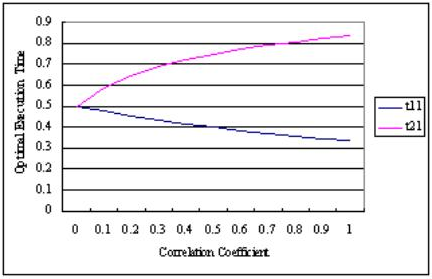
\includegraphics[width=10cm,height=6cm]{fg_s5n.png}
\end{center}
\caption[Optimal execution times for two stocks]{{\bf Optimal execution times for two stocks.}
 \quad This graph shows $t_{11}^*$ and $t_{21}^*$ for different price correlations when $W_1\sigma_1=0.2$,
 $W_2\sigma_2=0.1$,
and $T=1$.
 If $\rho_{12}=0$, optimal execution times coincide with the solution optimized independently
 ($t_{11}^*=t_{21}^*=0.5$).
 If $\rho_{12}>0$, optimal execution times are spread over the trading period according to correlation.
 In this case, the adjustment will be larger for the stock with the smaller $W\sigma$.}\label{fg_s5}
\end{figure}


Figure \ref{fg_s6} shows the standard deviation of VWAP execution errors.  Evidently the VWAP execution error becomes smaller when execution times are spread out, considering the portfolio effect.  It is interesting to note that although the total risk of a portfolio with a positive correlation is larger than that without correlation, this is not the case for VWAP execution risk.

\begin{figure}[htbp]
\begin{center}
 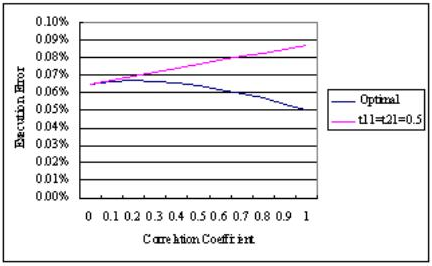
\includegraphics[width=10cm,height=6cm]{fg_s6n.png}
\end{center}
\caption[Execution error for two stocks]{{\bf Execution error for two stocks.}
 \quad This graph shows the standard deviation of VWAP execution errors ($y$-axis) for different price correlations
($x$-axis).
 Evidently the VWAP execution error becomes smaller when execution times are spread, considering the portfolio
effect.
 It is interesting to note that although the total risk of a portfolio with a positive correlation is larger
than that without correlation, this is not the case for VWAP execution risk.}\label{fg_s6}
\end{figure}


%%%%%%%%%%%%%%%%%%%%
\section{Closing Remarks}\label{sec_s5}
This chapter derives the static optimal execution strategy of a VWAP trade that minimizes the expected squared execution error.  This method is powerful because the optimal execution strategy is determined by an iteration of a single variable optimization, rather than by a multivariable optimization.  Analytical solutions are derived in some cases.  The following results are obtained through our analysis.  For a single-stock trade, if price volatility is independent of market trading volume, the optimal execution strategy is determined only by the expected market trading volume distribution and is independent of expectations regarding the magnitude and time dependency of price volatility.  If price volatility is positively correlated with market trading volume, optimal execution times turn out to lag behind the expected market trading volume distribution.  This is because once price volatility and market trading volume surge, traders have to make considerable trades to track market trading volume while execution times do not matter when these parameters remain small throughout the day.  In a basket trade, execution error can be reduced by spreading out execution times according to the correlation of price movement.  Further, we examine these theoretical results with actual trading data and simulations.

This chapter focuses on static optimization since observed variables such as price volatility and the market trading volume of small orders with low liquidity may contain statistical errors too large to be used in forecasting, and there are some concerns that dynamic optimization is inaccurate.  However, we might be able to predict the behavior of stocks with frequent trades to some extent, and dynamic optimization may reduce execution error further in such cases.  Dynamic optimization is analyzed in Chapter \ref{chap_d}.

For simplicity, this chapter minimizes execution error caused by price movement.  In the real world, however, the direct cost of market impact and the indirect cost of information leakage are certainly significant factors in a VWAP trade.  This issue is left for further analysis.


%%%%%%%%%%%%%%%%%%%%%%%%
\section{Appendix}\label{sec_sappendix}

\subsection{Proof of Proposition \ref{prop_s1}}
The expected square error of the whole VWAP transaction is
\begin{eqnarray*}
   \ex{(VWAP-vwap)^2}
    & = & \ex{\left(\frac{\int_0^T P(s)dV(s)+v(T) \times vwap}{V(T)+v(T)}-vwap\right)^2} \\
    & = & \ex{\left(\frac{\int_0^T P(s)dV(s)-V(T) \times vwap}{V(T)+v(T)}\right)^2} \\
    & = & \ex{\left\{\left(\frac{V(T)}{V(T)+v(T)}\right)\left(\frac{\int_0^T P(s)dV(s)}{V(T)}-\frac{\int_0^T P(s)dv(s)}{v(s)}\right)\right\}^2}.
\end{eqnarray*}
Since $P(s)=\int_0^s dP(t)+P(0)$,
\begin{eqnarray*}
  \int_0^T P(s)dV(s)
  & = & \int_0^T \int_0^s dP(t)dV(s) +\int_0^T P(0)dV(s) \\
  & = & \int_0^T \int_t^T dV(s)dP(t) + P(0)V(T).
\end{eqnarray*}

So,
\begin{eqnarray*}
  \frac{\int_0^T P(s)dV(s)}{V(T)}
  & = & \frac{\int_0^T \int_t^T  dV(s)dP(t)+P(0)V(T)}{V(T)} \\
  & = & \frac{\int_0^T \{V(T)-V(t)\}dP(t)}{V(T)}+P(0)\\
  & = & \int_0^T X(t)dP(t)+P(0).
\end{eqnarray*}
Therefore, the equation above becomes
\begin{eqnarray*}
   &   & \ex{\left\{\left(\frac{V(T)}{V(T)+v(T)}\right)\int_0^T (X(t)-x(t))dP(t)\right\}^2} \\
   & = & \ex{\left(\frac{V(T)}{V(T)+v(T)}\right)^2} \ex{\left\{ \int_0^T (X(t)-x(t))dP(t) \right\}^2} \\
   & & \hspace{2cm} +\cov{\left(\frac{V(T)}{V(T)+v(T)}\right)^2}{\left\{ \int_0^T (X(t)-x(t))dP(s) \right\}^2}.
\end{eqnarray*}

%%%%%%%%%%%%%%%%%
\subsection{Proof of Proposition \ref{prop_s2}}
\begin{eqnarray*}\label{eq_s14}
  \lefteqn{\min\int_0^T \{-2\ex{\sigma(t,V)^2X(t)}x(t)+ \ex{\sigma(t,V)^2}x(t)\}dt} \\
    & = & \min \sum_{k=1}^{v(T)} \int_{t_{k-1}}^{t_k} \{-2 \ex{\sigma(t,V)^2X(t)}x(t)+ \ex{\sigma(t,V)^2}x(t)^2\}dt.
\end{eqnarray*}
The first term is calculated as
\begin{eqnarray*}
  \lefteqn{\sum_{k=1}^{v(T)} \int_{t_{k-1}}^{t_k} \{-2\ex{\sigma(t,V)^2X(s)}x(t)\}dt} \\
    & = & \sum_{k=1}^{v(T)} \int_{t_{k-1}}^{t_k} \left\{-2\ex{\sigma(t,V)^2X(s)}\left(1-\frac{k-1}{v(T)} \right) \right\} dt\\
    & = & \sum_{k=1}^{v(T)} (v(T)-k+1)\int_{t_{k-1}}^{t_k} \left\{-\frac{2
\ex{\sigma(t,V)^2X(s)}}{v(T)}\right\}dt\\
    & = & \sum_{k=1}^{v(T)-1} (v(T)-k)\int_{t_{k-1}}^{t_k} \left\{-\frac{2\ex{\sigma(t,V)^2X(s)}}{v(T)}\right\}dt+\int_0^{t_v} \left\{-\frac{2\ex{\sigma(t,V)^2X(s)}}{v(T)}\right\}dt \\
    & = & \sum_{k=1}^{v(T)-i} (v(T)-k+1-i)\int_{t_{k-1}}^{t_k} \left\{-\frac{2\ex{\sigma(t,V)^2X(s)}}{v(T)} \right\}dt+\sum_{k=v(T)+1-i}^{v(T)} \int_0^{t_k} \left\{-\frac{2\ex{\sigma(t,V)^2X(s)}}{v(T)}\right\}dt \\
    & = & \sum_{k=1}^{v(T)} \int_0^{t_k} \left\{-\frac{2\ex{\sigma(t,V)^2X(s)}}{v(T)}\right\}dt.
\end{eqnarray*}
Also, the second term becomes
\begin{eqnarray*}
   \lefteqn{\sum_{k=1}^{v(T)} \int_{t_{k-1}}^{t_k} \{ \ex{\sigma(t,V)^2}x(t)^2\}dt}\\
    & = & \sum_{k=1}^{v(T)} \int_0^{t_k} \ex{\sigma(t,V)^2}x(t_{k-1})^2 dt-\sum_{k=1}^{v(T)} \int_0^{t_{k-1}} \ex{\sigma(t,V)^2}x(t_{k-1})^2 dt\\
    & = & \sum_{k=1}^{v(T)} \int_0^{t_k} \ex{\sigma(t,V)^2}x(t_{k-1})^2 dt-\sum_{k=1}^{v(T)-1} \int_0^{t_k} \ex{\sigma(t,V)^2}x(t_k)^2 dt\\
    & = & \sum_{k=1}^{v(T)} \int_0^{t_k} \{ \ex{\sigma(t,V)^2}x(t_{k-1})^2\}dt\\
    &   & -\left[ \sum_{k=1}^{v(T)} \int_0^{t_k} \ex{\sigma(t,V)^2}x(t_k)^2 dt+\int_0^{t_0} \ex{\sigma(t,V)^2}x(t_0)^2 dt-\int_0^{t_v} \ex{\sigma(t,V)^2}x(t_v)^2 dt \right]\\
    & = & \sum_{k=1}^{v(T)} \int_0^{t_k} \ex{\sigma(t,V)^2} \{ x(t_{k-1})^2-x(t_k)^2 \}dt\\
    & = & \sum_{k=1}^{v(T)} \int_0^{t_k} \ex{\sigma(t,V)^2} \left\{ \left(\frac{v(T)-k+1}{v(T)}\right)^2-\left(\frac{v(T)-k}{v(T)}\right)^2 \right\} dt\\
    & = & \sum_{k=1}^{v(T)} \int_0^{t_k} \ex{\sigma(t,V)^2}\frac{2(v(T)-k)+1}{v(T)^2} dt.
\end{eqnarray*}
Therefore, (\ref{eq_s14}) becomes
\[
  \min \sum_{k=1}^{v(T)} \int_0^{t_k} \left\{ -\frac{2 \ex{\sigma(t,V)^2X(t)}}{v(T)
\ex{\sigma(t,V)^2}}+\frac{2(v(T)-k)+1}{v(T)^2}\right\} \ex{\sigma(t,V)^2} dt.
\]

%%%%%%%%%%%%%%%%%
\subsection{Proof of Proposition \ref{prop_s3}}
Since $X(t)$ and $x(t)$ are uncorrelated, (\ref{eq_s5}) becomes
\[
  \min \sum_{k=1}^v \int_0^{t_k} \left\{-\frac{2\ex{X(t)}}{v(T)}+\frac{2(v(T)-k)+1}{v(T)^2} \right\}\ex{\sigma(t)^2}dt.
\]
If we represent the integrand as $f_k(t)$, we can prove that this function takes a negative value in $[0,t_{k-1}]$ and turns from negative to positive just once in $[t_{k-1},T]$, and therefore, we can choose $\{t_k^*\}$ at such point.  This is because the function is monotone increasing with respect to $t$, and the sign of the integrand can be checked by 

\[
  \begin{array}{ll}
    \displaystyle f_1(0)=-\frac{1}{v(T)^2}<0, \\
    \displaystyle f_1(T)=\frac{2v(T)-1}{v(T)^2}>0
  \end{array}
\]
when $k=1$.  Also, assuming that the relationship holds for $k-1$, it can be proved for $k$ also since
\[
  \begin{array}{ll}
    \displaystyle f_k(t_{k-1}^*)=f_{k-1}(t_{k-1}^*)-\frac{1}{v(T)^2}<f_{k-1}(t_{k-1}^*) \leq 0, \\
    \displaystyle f_k(T)=\frac{2(v(T)-k)+1}{v(T)}>0.
  \end{array}
\]
So, the relationship holds for all $k$. 
Therefore, $\{t_k^*\}$ is determined to satisfy
\[
  -\frac{2\ex{X(t_k^*)}}{v(T)}+\left\{ \frac{v(T)-k+1}{v(T)} \right\}^2- \left\{ \frac{v(T)-k}{v(T)} \right\}^2 \leq 0,
\]
and
\[
  \lim_{t \downarrow t_k^*} -\frac{2\ex{X(t_k)}}{v(T)}+\left\{ \frac{v(T)-k+1}{v(T)} \right\}^2-
\left\{ \frac{v(T)-k}{v(T)} \right\}^2 \geq 0.
\]
Solving this equation, 
\[
  \ex{X(t_k^*)} \geq \frac{2(v(T)-k)+1}{2v(T)} \geq \lim_{t \downarrow t_k^*} \ex{X(t)}.
\]
We then first assume that $E[X(t)]$ is continuous at $t_k^*$.  In this case, 
\[
  \ex{X(t_k^*)}=\frac{2(v(T)-k)+1}{2v(T)}.
\]
Also, from (\ref{eq_s4}),
\[
  x(t_k^*)=1-\frac{k}{v(T)}=\frac{2v(T)\ex{X(t_k^*)}+1}{2v(T)}.
\]
According to Figure \ref{fg_s1}, $x^*(t)$ takes a constant value over the $t$ range of 
\[
  \ex{X(t_k^*)}-\frac{1}{v(T)}< \ex{X(t)} \leq \ex{X(t_k^*)}
\]
which is equivalent to
\[
  \ex{X(t)} \leq \ex{X(t_k^*)} < \ex{X(t)}+\frac{1}{v(T)}.
\]
Therefore, 
\[
  \frac{2v(T)\ex{X(t)}-1}{2v(T)} \leq x^*(t) < \frac{2v(T)\ex{X(t)}+1}{2v(T)}.
\]
Or equivalently,
\[
  x^*(t)=\frac{\lfloor (2v(T)\ex{X(t)}+1)/2 \rfloor}{v(T)}.
\]
Next, if $\ex{X(t)}$ is not continuous at $t_k^*$, the same argument can be applied.  Specifically, 
\[
  x^*(t_k^*)=\frac{\lfloor (2v(T)\ex{X(t_k^*)}+1)/2 \rfloor}{v(T)}
\]
from left continuity, and also,
\[
  \lim_{t \downarrow t_k^*}x^*(t)=\lim_{t \downarrow t_k^*}\frac{\lfloor (2v(T)\ex{X(t)}+1)/2 \rfloor}{v(T)}.
\]
Therefore, we can conclude that for all $t$,
\[
  x^*(t)=\frac{\lfloor (2v(T)\ex{X(t)}+1)/2 \rfloor}{v(T)}.
\]

%%%%%%%%%%%%%%%%%
\subsection{Proof of Proposition \ref{prop_s5}}
\begin{eqnarray*}
  \lefteqn{\min\sum_{i=1}^N \sum_{j=1}^N W_{ij}\int_0^T \ex{\rho_{ij}\sigma_i\sigma_j(X_i-x_i)(X_j-x_j)}dt}\\
    & = & \min \left[ \sum_{i=1}^N \sum_{j=1}^N W_{ij}\int_0^T \{-\ex{\rho_{ij}\sigma_i\sigma_jX_i}x_j-\ex{\rho_{ij}\sigma_i\sigma_jX_j}x_i+\ex{\rho_{ij}\sigma_i\sigma_j}x_ix_j\}dt \right.\\
    &   & \left. +\sum_{i=1}^N \sum_{j=1}^N W_{ij}\int_0^T \ex{\rho_{ij}\sigma_i\sigma_jX_iX_j}dt \right]\\
    & = & \min \left[ \sum_{i=1}^N \sum_{j=1}^N W_{ij} \sum_{k=1}^{v_i(T)}\int_0^{t_{ik}} \left\{-\frac{2\ex{\rho_{ij}\sigma_i\sigma_jX_j}}{v_i\ex{\rho_{ij}\sigma_i\sigma_j}} \right\} \ex{\rho_{ij}\sigma_i\sigma_j}dt+\int_0^T \ex{\rho_{ij}\sigma_i\sigma_j}x_ix_jdt \right.\\
    &   & \left. +\sum_{i=1}^N \sum_{j=1}^N W_{ij}\int_0^T \ex{\rho_{ij}\sigma_i\sigma_jX_iX_j}dt. \right]
\end{eqnarray*}
Because each series of $\{t_{ik}\}$ is double counted in the series of $\{t_k^{ij}\}$,
\begin{eqnarray*}
  \lefteqn{\min \left[ \sum_{i=1}^N \sum_{j=1}^N W_{ij} \left\{ \sum_{k=1}^{v_i(T)}\int_0^{t_{ik}} \left(-\frac{2\ex{\rho_{ij}\sigma_i\sigma_jX_j}}{v_iE[\rho_{ij}\sigma_i\sigma_j]}\right)\ex{\rho_{ij}\sigma_i\sigma_j}dt \right. \right.} \\
    &   & \left. \left. +\sum_{k=1}^{v_i(T)+v_j(T)}\int_0^{t_k^{ij}}\frac{x_i(t_{k-1}^{ij})x_j(t_{k-1}^{ij})-x_i(t_k^{ij})x_j(t_k^{ij})}{2} \ex{\rho_{ij}\sigma_i\sigma_j}dt \right\} \right]\\
    &   & +\sum_{i=1}^N \sum_{j=1}^N W_{ij}\int_0^T \ex{\rho_{ij}\sigma_i\sigma_jX_iX_j}dt \\
    & = & \min \sum_{i=1}^N \sum_{j=1}^N W_{ij} \sum_{k=1}^{v_i(T)+v_j(T)} \int_0^{t_k^{ij}} \left\{ -\frac{\ex{\rho_{ij}\sigma_i\sigma_jX_j}}{v_i \ex{\rho_{ij}\sigma_i\sigma_j}}+\frac{x_i(t_{k-1}^{ij})x_j(t_{k-1}^{ij})-x_i(t_k^{ij})x_j(t_k^{ij})}{2}\right\}\ex{\rho_{ij}\sigma_i\sigma_j}dt \\
    &   & +\sum_{i=1}^N \sum_{j=1}^N W_{ij}\int_0^T \ex{\rho_{ij}\sigma_i\sigma_jX_iX_j} dt.
\end{eqnarray*}
